\chapter{BAA TRAINING VIETNAM DESCRIPTION AND STRUCTURE}

\renewcommand{\headrulewidth}{0.5pt}
\renewcommand{\footrulewidth}{0.5pt}
\thispagestyle{plain}
\pagestyle{fancy}
\fancyhf{}
\fancyhead[L]{\textbf{CHAPTER 2}}
\fancyhead[R]{\textbf{Graduate Report}}
\raggedright
\fancyfoot[L]{From: Nguyen Van Anh Tuan}
\fancyfoot[R]{Page \thepage}

\justifying

\section{Registration and address}
    On February 2nd, 2018 BAA Training Vietnam was registered, assigned company number 0314876711. \\
    \begin{figure}[H]
        \centering
        
\includegraphics[width=0.6\linewidth]{img/company-logo.png}
        \caption{BAA Training Vietnam logo}
    \end{figure}
    BAA Training Vietnam shall maintain a principle business office that is physically located at the address shown on the ATO certificate. \\ 
    \vspace{3mm}
    The principle business office may not be shared with, or used by, another person who holds an ATO certificate.
    \begin{itemize}
        \item \textbf{Address:} 99 Le Van Viet street, Tang Nhon Phu A ward, District 9, Ho Chi Minh city, postal address 71207
        \item \textbf{Hotline:} +84 28 389 739 39
        \item BAA Training Vietnam is CAAV approved ATO providing EASA standard aviation training solutions in Asia-Pacific region.
    \end{itemize}
    \begin{figure}[H]
        \centering
        
\includegraphics[width=0.6\linewidth]{img/company.jpg}
        \caption{Headquarter of BAA Training Vietnam}
    \end{figure}

\section{Field Of Activities}
    BAA Training Vietnam's facilities and working environment shall be appropriate for the task to be performed and be acceptable to the Authority. \\
    \vspace{3mm}
    BAA Training Vietnam shall provide facilities, equipment, and material equal to the standards currently required for the issue of the certificate 
    and rating that it holds. \\
    \vspace{3mm}
    BAA Training Vietnam have, or have access to, the necessary information, equipment, training devices and material to conduct the courses for which 
    the organization is approved. \\
    \vspace{3mm}
    BAA Training Vietnam may not make a substantial change in facilities, equipment, or material that have been approved for a particular curriculum, 
    unless that change is approved by the Authority in advance. \\
    \vspace{3mm}
    The BAA Training Vietnam shall have a technical library adequate for the level of training conducted. \\ 
    \vspace{3mm}
    BAA Training Vietnam is Approved Training Organization with the privilege to advertise and provide approved training courses as listed in the ATO 
    certificate in a location that is normally accessible to the public and that is not obscured. \\
    \vspace{3mm}
    BAA Training Vietnam may provide training only if: 
    \begin{itemize}
        \item The Training Organization is accredited for such activities (the permission is indicated in the attachment to ATO Certificate Training Course 
        Approval);
        \item Has a relevant training program approved by CAAV;
        \item Has a sufficient number of ground and flight instructors (if necessary);
        \item Has necessary training material and equipment for the training course.
    \end{itemize}

\section{Premises}
    The ATO holder shall show that the classrooms and briefing facilities:
    \begin{itemize}
        \item Used for instructional purposes are heated, lighted, and ventilated to conform to local building, sanitation, and health codes;
        \item Are not routinely subject to significant distractions caused by flight operations and maintenance operations at the aerodrome;
        \item Audio and visual training equipment appropriate to the training conducted, including computer projected documents. 
    \end{itemize}
    \subsection{Building In}
        BAA Training Vietnam has 1 building located in district 9, Ho Chi Minh city. The building is framed, insulated and covered with lightweight metal 
        sheets from the outside. These training premises occupy two floors and cover the area of approximately 200 $m^2$. \\
        \vspace{3mm}
        The first floor includes:
        \begin{itemize}
            \item 1 real size A320 flight simulators, their maintenance, spare part store and technical rooms;
            \item 1 Archive room;
            \item 4 Classrooms;
            \item 1 Pantry room;
            \item 1 Meeting room.
        \end{itemize}
        The second floor includes:
        \begin{itemize}
            \item 4 Office rooms;
            \item 5 Briefing room;
            \item 1 ATP training room; 
            \item 5 Classrooms;
            \item 1 Lounge room.
        \end{itemize}
        The majority of rooms have windows. In addition to the natural light, all rooms have led/fluorescent lamps. All rooms are ventilated and equipped 
        with air conditioners; supplied with 220V/50 Hz electricity and have the Internet connection. There are also backboards, projectors and aircraft 
        cabin models (if necessary).
    \subsection{Training Equipment}
        \subsubsection{Flight Simulation Training Devices}
            Flight simulation training devices shall be qualified according to requirements prescribed by the Authority. \\
            \vspace{3mm}
            The use of flight simulation training devices shall be approved by the Authority to ensure that they are appropriate to the task. \\ 
            \vspace{3mm}
            BAA Training Vietnam shall have available exclusively, for adequate periods of time and at a location approved by the Authority, adequate flight 
            training equipment and courseware, including at least one flight simulation training device suitable for the approved curriculum. \\ 
            \vspace{3mm}
            BAA Training Vietnam shall show that each flight simulation training device used for training, testing, and checking will be or is specifically 
            qualified and approved by the Authority for:
            \begin{itemize}
                \item Each manoeuvre and procedure for the make, model, and series of aircraft, set of aircraft, or aircraft type simulated, as applicable;
                \item Each curriculum or training course in which the flight simulation training device is used, if that curriculum or course is used to satisfy 
                any requirements of these regulations.
            \end{itemize}
            BAA Training Vietnam shall ensure, prior to use, that the approval required by this section includes:
            \begin{itemize}
                \item The set of aircraft or type aircraft;
                \item If applicable, the particular variation within type for which the training, testing, or checking is being conducted;
                \item The particular manoeuvre, procedure, or crew memeber function to be performed.
            \end{itemize}
            The ATO holder shall ensure that each flight simulation training device used is:
            \begin{itemize}
                \item Maintenanced to ensure the reliability of the performances, functions, and all the other characteristics that were required for qualification;
                \item Modified to conform with any modification to the aircraft being simulated if the modifications results in changes to performance, function, or 
                other characteristics required for qualification;
                \item Given a functional preflight check each day before being used;
                \item Provided with a discrepancy log in which the instructor or evaluator, at the end of each training session, enters each discrepancy.
            \end{itemize}
    \subsection{Other Training Devices}
        In order to conduct the training, BAA Training Vietnam uses the other following training equipment:
        \begin{itemize}
            \item CAE 400XR Flight Training Device;
            \item Personal computers and tablet computers;
            \item Computer projector with remote control;
            \item Computers with headphones and microphones sets, software and sound recordings, radio contact for training and further self-development.
        \end{itemize}

\section{Approved Training Organization (ATO) Organizational Structure}
    \begin{figure}[H]
        \centering
        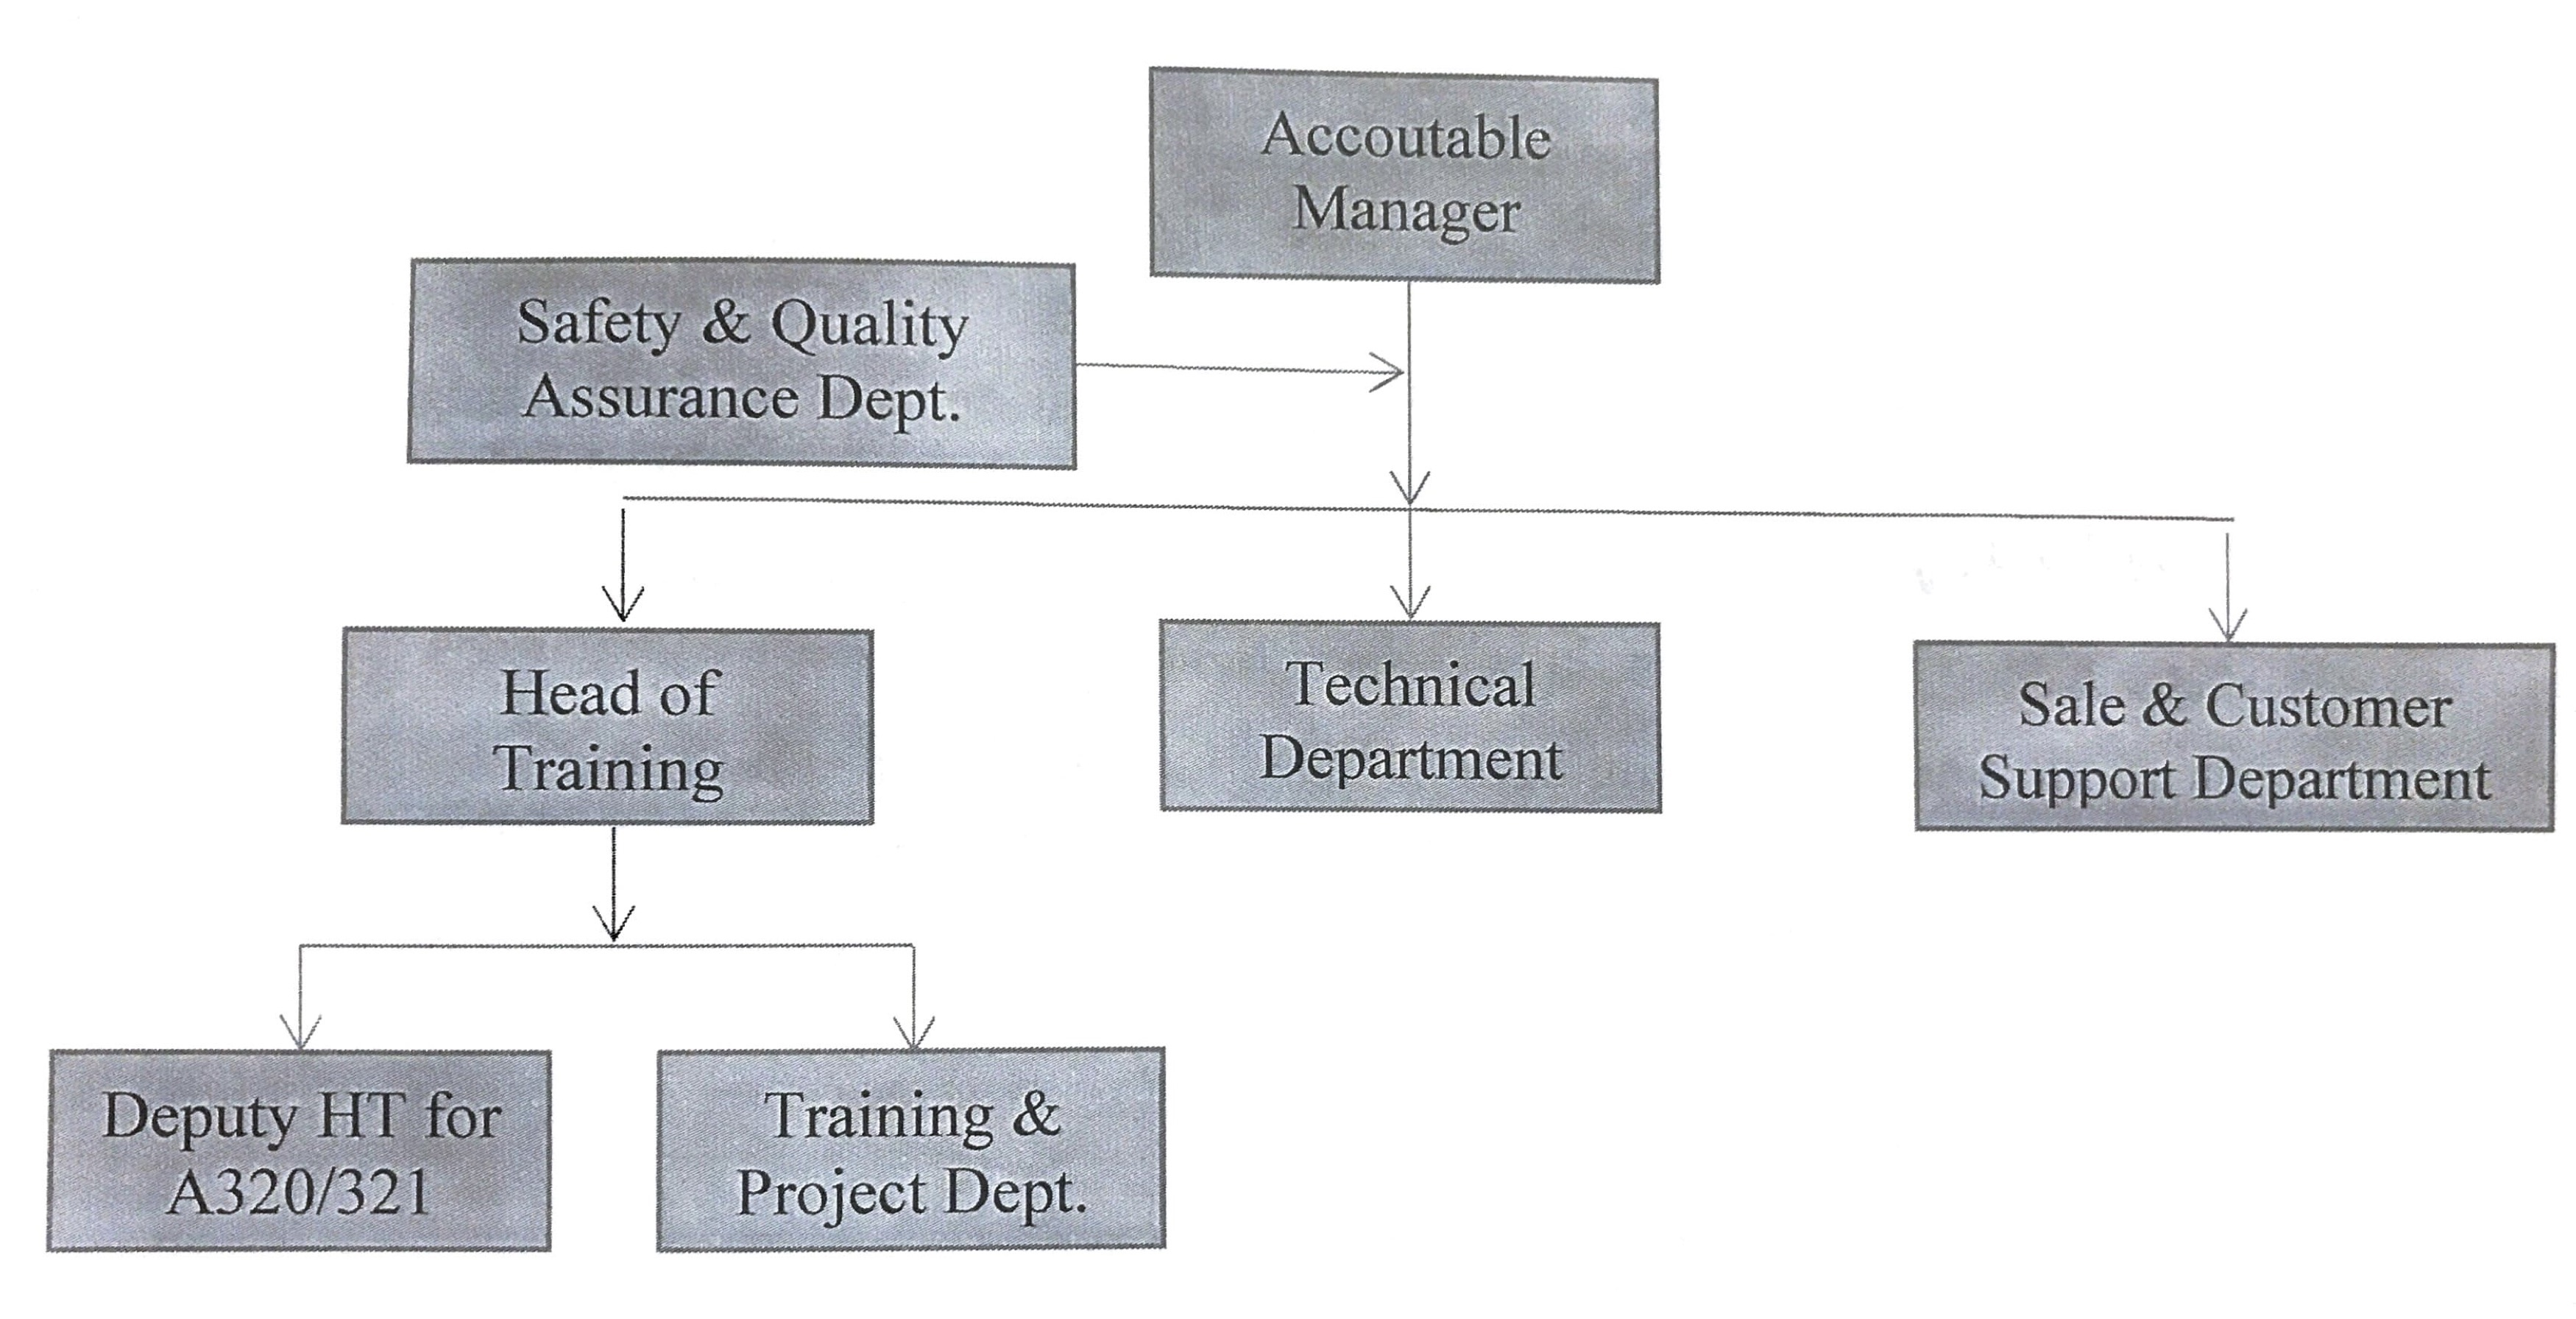
\includegraphics[width=0.6\linewidth]{img/structure.jpg}
        \caption{BAA Training Vietnam Organizational Structure}
    \end{figure}
    \subsection{Managing Director}
        To be the legal representative of BAA Training Vietnam on the legal side, to sign the contract and to be the spokesperson for the company. \\ 
        \vspace{3mm}
        Responsible for managing all business activities to ensure that these activities comply with the provisions of Vietnamese law, the guidance 
        of the Ministry of Transport, the Civil Aviation Administration of Vietnam as well as legal documents. \\ 
        \vspace{3mm}
        At the same time, he is responsible for running the company's activities, reviewing and recruiting personnel and appointing the positions of 
        Heads of Training, Technical, Sales and Customer Care departments. \\ 
        \vspace{3mm}
        In addition, the CEO also performs other obligations and powers specified in the company's internal documents.
    \subsection{Quality Assurance Department}
        The main task is to ensure that the company's activities always comply with the quality regulations issued by BAA Training Vietnam internally 
        and required by the Civil Aviation Authority of Vietnam. \\ 
        \vspace{3mm}
        Along with that, it is a tool to support the CEO in formulating policies and standards for aviation training, company operation or human 
        resource quality.
    \subsection{Training Department}
        Develop training standards according to the requirements specified in the aviation safety regulations - Section 7 on Airline Officer Licenses. \\ 
        \vspace{3mm}
        Responsible for training, training students and supervising the company's training program to ensure service quality, detect hazards in the 
        process of operation. \\
        \vspace{3mm}
        BAA Training Department includes: 
        \begin{itemize}
            \item Head of training
            \item Flight instructor
            \item Ground instructor
            \item Training and service development department
        \end{itemize}
    \subsection{Technical Department}
        Ensure that the training equipment at the company meets technical standards and is always in stable condition through regular inspection and 
        evaluation activities. When detecting errors, they must notify the Executive Director for timely resolution. In addition, the technical department 
        is also responsible for preparing equipment for students before the lesson begins.
    \subsection{Sales And Customer Care Department}
        Consulting and supporting students to learn information about the company's services. Answer questions and complaints of students during the learning 
        process. Support students when needed and manage the company's social networking sites to reach and attract new students.

\section{Performance results 2019 - 2020}
    Participating in the Vietnamese market since 2018 but BAA Training Vietnam officially went into operation in 2019 after completing the construction 
    and assembling of equipment. Therefore, the operation time of the center up to now is less than 2 years. However, the operating results of BAA 
    Training Vietnam still have a good signal. \\ 
    \vspace{3mm}
    In the past year 2020, BAA Training Vietnam was granted the UPRT training certificate - Upset Prevention and Recovery Training for the first A320 
    airplane in Vietnam for the purpose of improving the pilot's ability as well as the level of flight safety during flight performance.

\section{Job Description At The Internship Company}
    At the internship company, I was able to participate in an internship at the technical department as a flight simulator maintenance engineer. At that place, 
    i was able to read and participate in observing the flight simulator in action and I also observed the tasks that the maintenance engineers there performed 
    during each maintenance, and understand what maintenance is like on a flight simulator and what to do.